\begin{figure}[!ht]
  \centering
  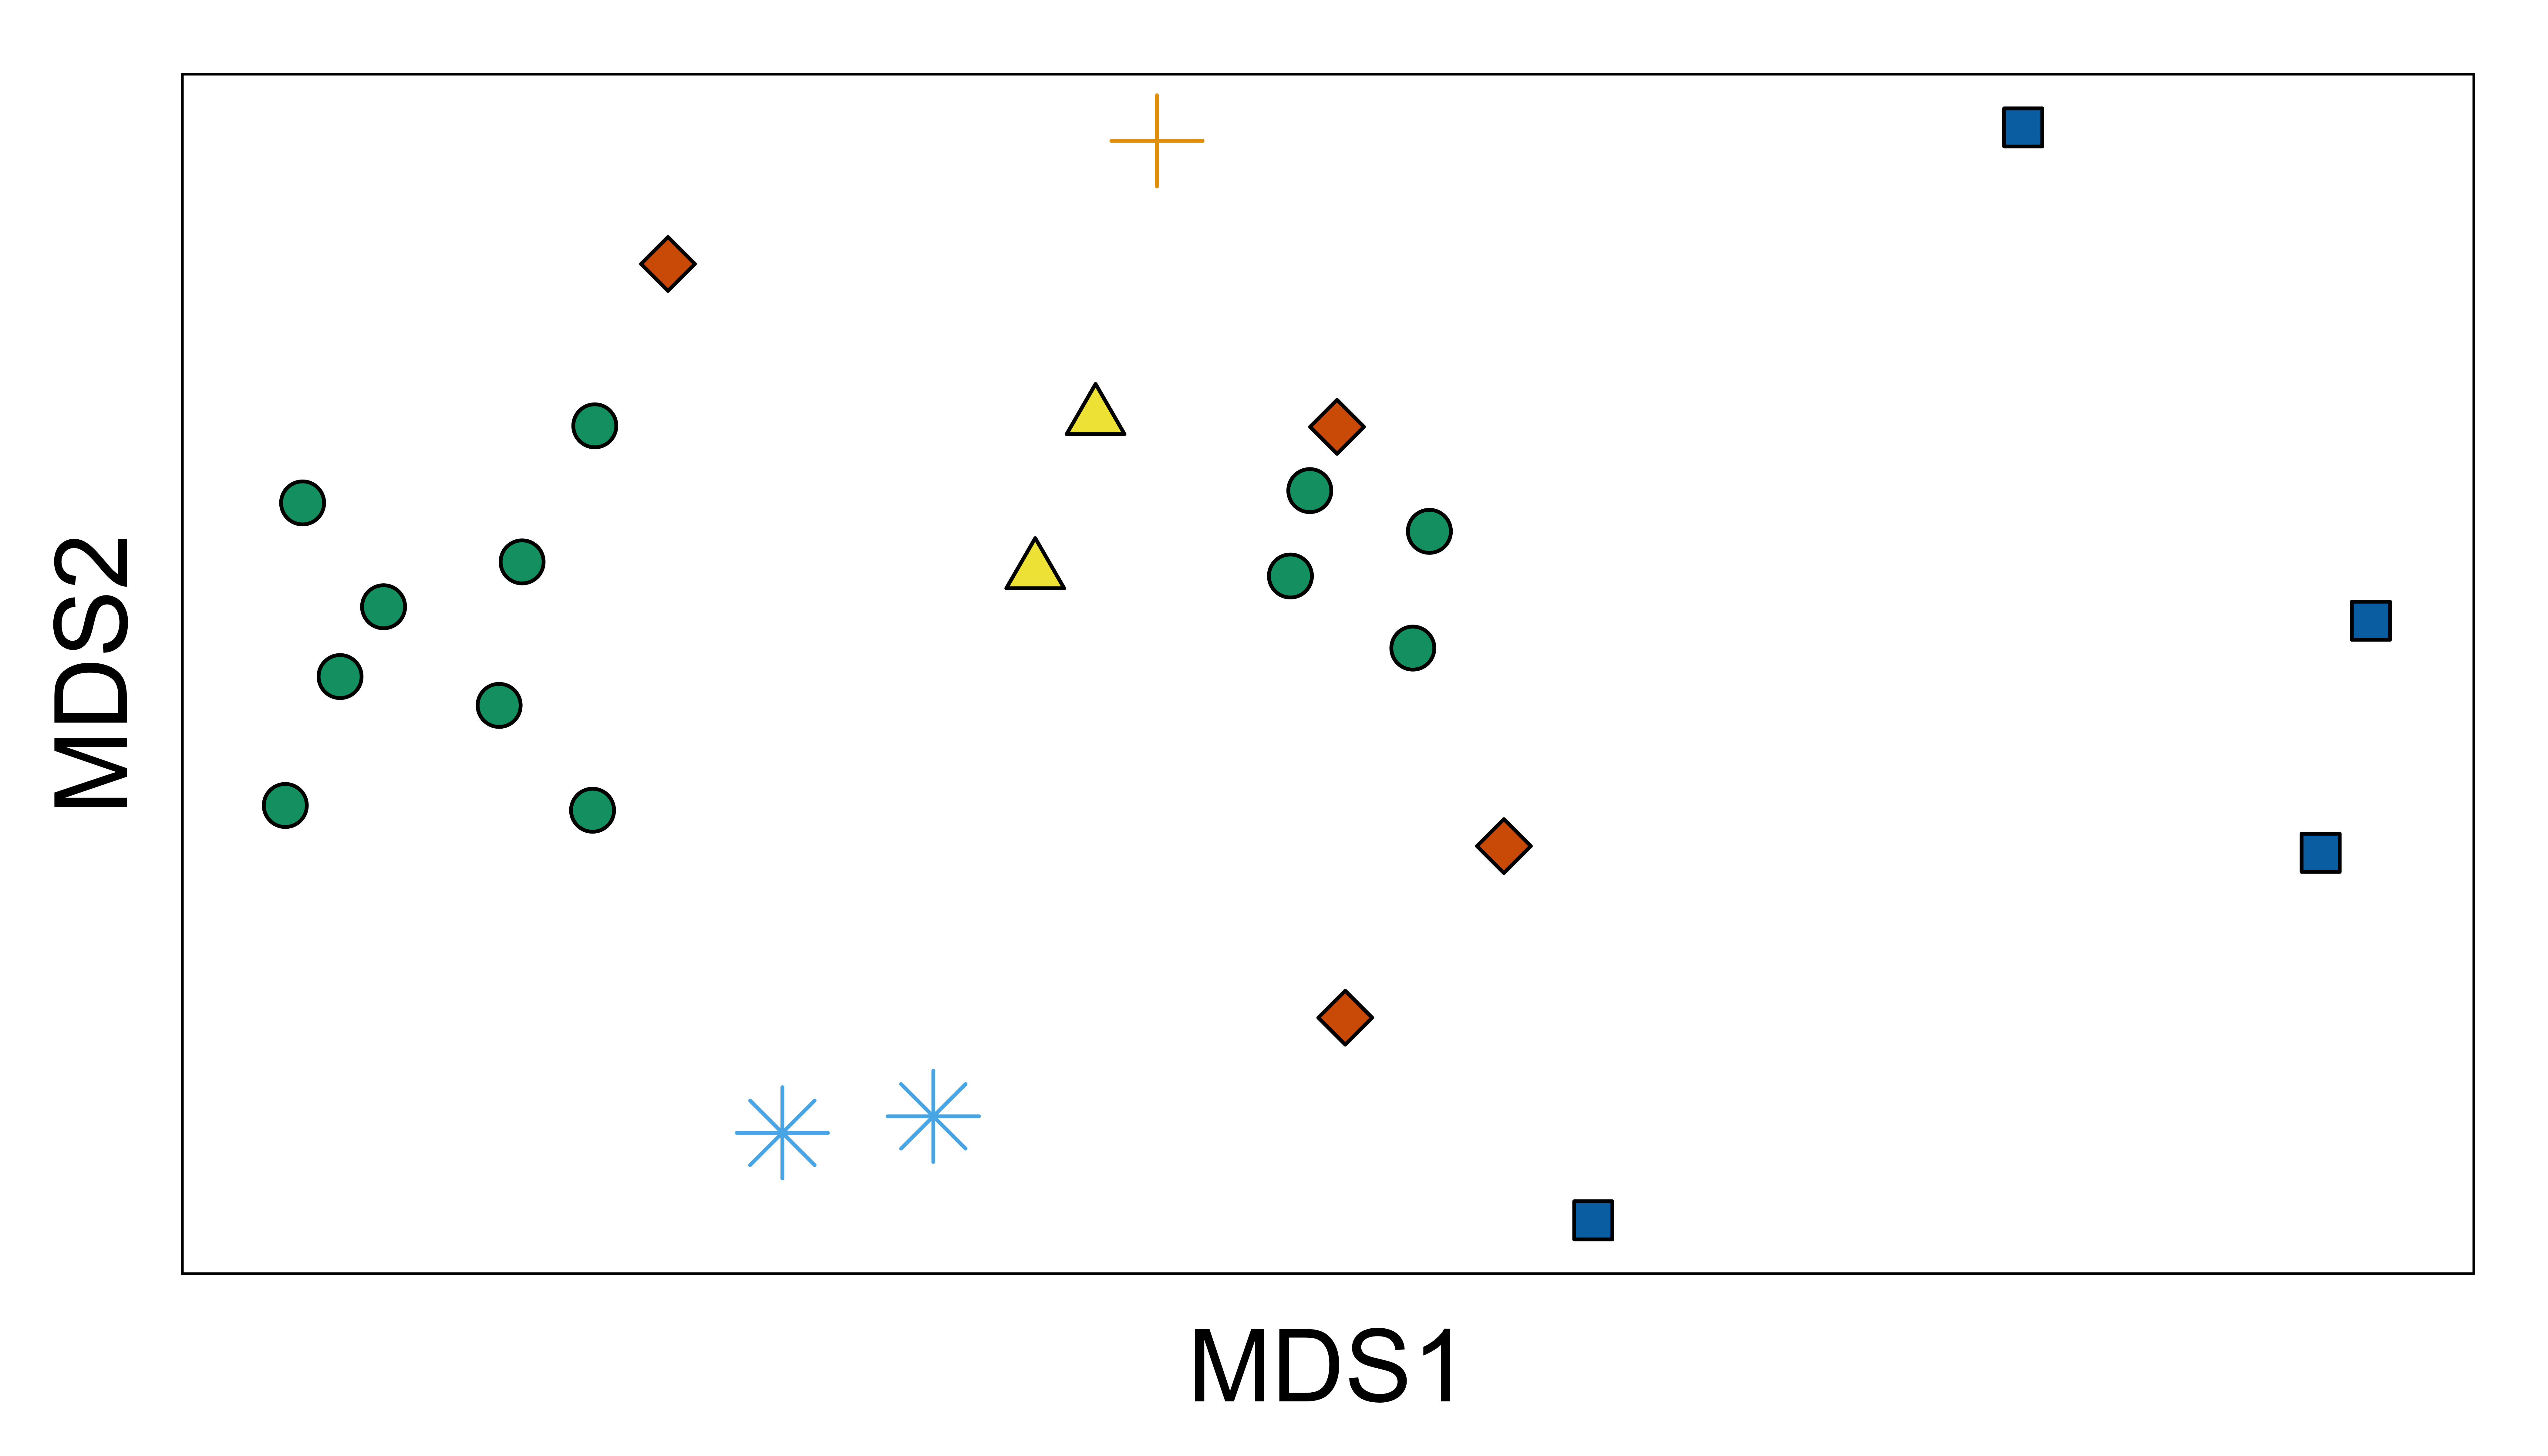
\includegraphics[width=\textwidth]{../advection/nMDSadvection.png}
  \caption[nMDS of advective distances between samples.]{nMDS ordination of the advection distance matrix (2D stress = 0.19). Antarctic Intermediate Waters (AAIW), light blue stars; Subantarctic Mode Water (SAMW), orange crosses; Antarctic Bottom Water (AABW), dark blue squares; Antarctic Zone (AZ), green circles; Polar Frontal Zone (PFZ), yellow triangles; Circumpolar Deep Water (CDW), red diamonds.}
  \label{fig:nMDSadvection}
\end{figure}
